\chapter{Garment Depth Map Clustering}
\label{garment_clustering}

This chapter explains in detail the Garment Depth Map Clustering stage that our algorithm performs to the garment data that has been previously segmented to group similar height regions of the garment. Some of these clusters represent overlapped regions of the garment. The block diagram of this stage can be seen in Figure \ref{fig:garment_clustering_blocks}.

\begin{figure}[thpb]
    \centering
    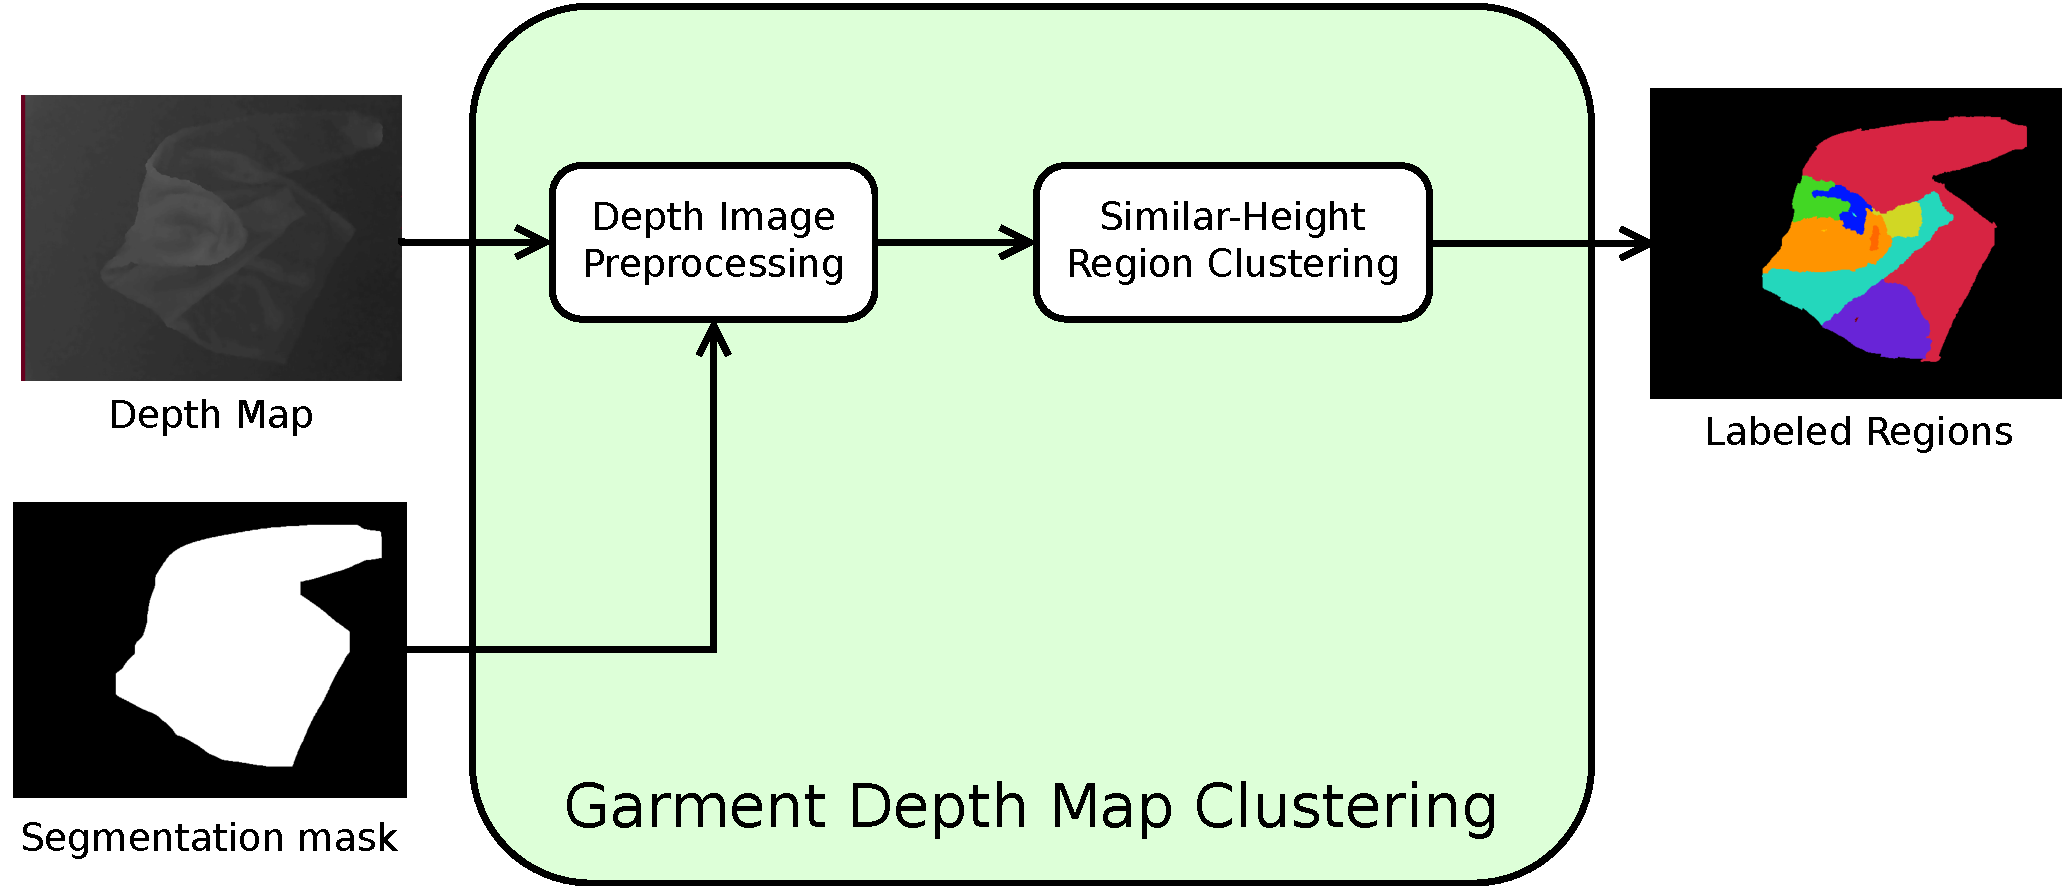
\includegraphics[width=0.98\textwidth]
    {figures/Garment-depthmap-diagram.pdf}
    \caption[Block diagram showing an overview of the Garment Depth Map Clustering stage and its different steps.]
    {Block diagram showing an overview of the Garment Depth Map Clustering stage and its different steps. The inputs of this stage are the depth map image and the segmentation mask obtained in the previous stage. These inputs are combined and preprocessed in order to apply the clustering step. The output of this stage are the labels of the different cluster regions.}
    \label{fig:garment_clustering_blocks}
\end{figure}

In this stage, the depth image data is preprocessed using the segmentation results from the previous stage to remove all depth data not related to the garment. Then, it applies a Watershed transform algorithm to find the different similar-height regions, that will be analyzed in the last stage to select the most suitable manipulation points to unfold the garment. 

As mentioned before, some of these regions of similar height correspond to overlappìng regions of the garment, whose order can be determined using the average depth value of the pixels in each region. The garment region with the lowerst height value then corresponds to the region of the garment underneath those overlapping regions.

Once the different regions are labeled, the labeled clusters are passed to the next stage in order to determine the uppermost fold and the most suitable unfolding direction.

\section{Depth Image Preprocessing}
\label{depth_image_preprocessing}

This step prepares the input depth data from the sensors to be used in later steps. The raw depth image data obtained from the robot RBG-D sensor cannot be used directly, as it contains data related to outliers and noise. The data coming from the table on which the garment lies is also present in this image. Therefore, this data requires some treatment before it can be processed in the next step (section \ref{garment_clustering_watershed}). 

For that purpose, the garment mask calculated in the previous stage, a required input of this step, is applied to the depth image of the garment. The objective is to discard the information related to the table. After this process only information about the garment is present on the depth image.

The depth input data is read expressed as a distance from the sensor to each pixel. As the next step will treat the depth data as a greyscale image, the remaining garment depth data needs to be normalized to the 8-bit range of a typical greyscale image. By normalizing the data we ensure that we are using the maximum resolution available (256 grey levels) to represent all the depth variability in the depth image. This helps the next step to find regions of similar height more accurately.

Figure \ref{fig:depth_map_preprocessing}  shows a comparison between the raw input depth data and the data after this processing step. The left image pixel values correspond to distances to the sensor expressed in mm, and the right image pixel values are those distances normalized to a 8-bit unsigned integer (256 values). The image on the left is shown mostly in grey shades, except from a thin red line seen on the left part of the image, corresponding to values out of sensor range. On the right image, representing the depth image after the preprocessing stage, it can be observed that the depth image now uses all the range available by the encoding as an 8-bit unsigned char.

\begin{figure}[htbp]
	\centering
    \begin{subfigure}[l]{0.495\textwidth}
	    \centering
    	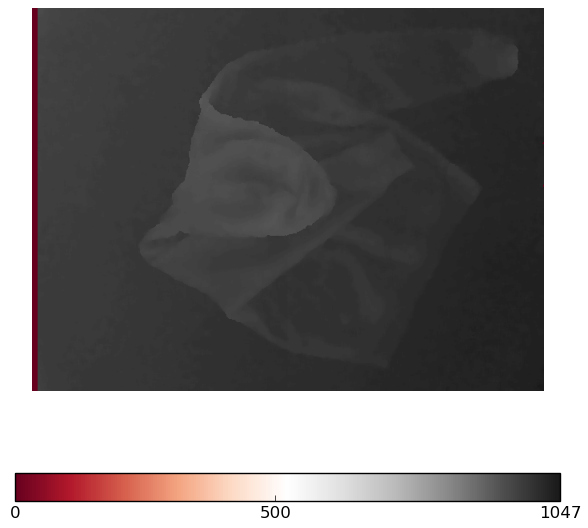
\includegraphics[width=\textwidth]
    	{figures/Depthmap-Raw-Depthmap-with-colorbar.png}
    	\caption{Before preprocessing}
	\end{subfigure}
	~
    \begin{subfigure}[r]{0.485\textwidth}
	    \centering
    	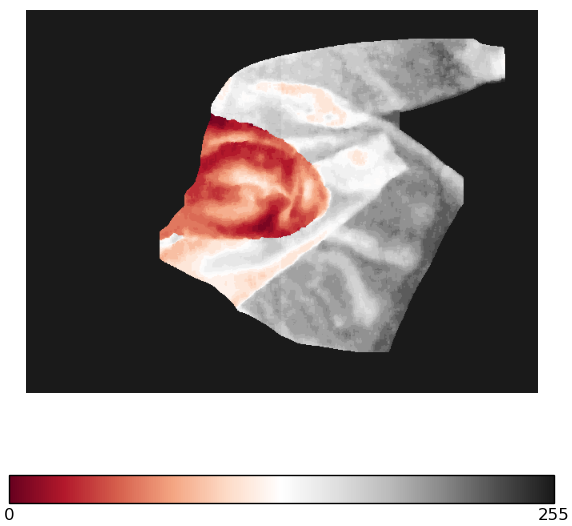
\includegraphics[width=\textwidth]
    	{figures/Depthmap-Normalized-Depthmap-with-colorbar.png}
    	\caption{After preprocessing}
    	\end{subfigure} 
    \caption[Depth image before and after preprocessing.]
    {Depth image before and after preprocessing. Note that pixels closer to the sensor are shown in red, and pixels further from the sensor are displayed in grey. White values are intermediate values. The correspondence between colors and distance is explained in the colorbar beneath each figure.} 
    \label{fig:depth_map_preprocessing}
\end{figure}


\section{Similar-Height Region Clustering}
\label{garment_clustering_watershed}

Once the garment depth data is separated from the table depth data and normalized in the previous step, regions of similar height must be identified and labeled.

Grouping points according to a common feature, such as height, is a clustering problem, and several clustering methods and alternatives were described in section \ref{architecture:depth_map_clustering}. A Watershed Transform \cite{digabel1978iterative} segmentation algorithm was selected to perform the clustering. This algorithm is faster than other superpixel approaches, and usually returns a single cluster per overlapping region, removing the need for a later merging step. This step is frequently required when working with superpixels to aggregate superpixels corresponding to similar regions, as they are conceived to divide the image in relatively small clusters of similar characteristics.

The Watershed Transform algorithm is a segmentation algorithm that considers a greyscale image as a topological surface where high intensity pixels correspond to peaks and hills, and low intensity pixels are equivalent to valleys. The algorithm fills the surface pouring water at each isolated valley. As the water level rises, the water from different sources will start to merge. To prevent them from merging, the algorithm constructs barriers at the merging regions, and continues this process of adding water and building barriers until all the peaks have been flooded. The resulting barriers are the segmentation regions border, and all the pixels within each region enclosed  by these borders correspond to a different segmented item. 

Figure \ref{fig:watershed_example} shows an example of applying the Watershed algorithm. The grey area represents a cross section of the image along a given image axis. Subfigure A shows the segmentation results when all local minima are selected as flooding sources (i.e. markers), and subfigure B shows the same results when one of those sources is omitted. The dotted lines on the right-hand side of the figure represent \pagebreak

\noindent the catchment basins resulting from the Watershed Transform, and the colored regions are the different segments obtained.

\begin{figure}[thbp]
    \centering
    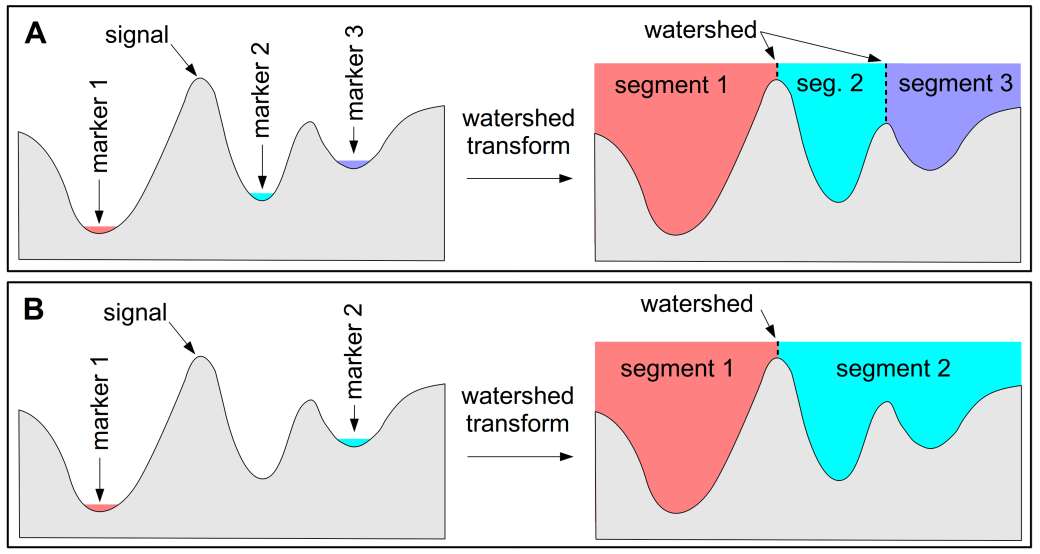
\includegraphics[width=\textwidth]
    {figures/watershed-example.png}
    \caption[Example of application of the Watershed Tranform algorithm]
    {Example of application of the Watershed Tranform algorithm. The grey area, marked as signal, represents the the pixel intensity along a given image direction, as if it was a cross section of the image. Figure extracted from \cite{rs6010776}.}
    \label{fig:watershed_example}
\end{figure}

A denoising process is performed before applying the Watershed transform, which is the actual clustering process. We use a Total Variation filter \cite{chambolle2004algorithm} to produce a smoother image while maintaining the edges sharp. The Total Variation filter works by minimizing the integral of the norm of the image gradient. As a result of this filter, piecewise-constant images (``cartoon-like'' images) are obtained. This denoising process is required when using the Watershed transform algorithm, as it is an algorithm highly sensitive to local minima, which can be present due to noise or irregularities in the image. 

The Watershed Transform segmentation algorithm is then applied to the depth image of the garment to locate the different parts that are overlapping each other. These regions are related to folded parts, that rest on top of other parts of the garment. 

\pagebreak
As said before, Watershed is very sensitive to local minima. Therefore, in practice, using local minima as sources for flooding leads to over-segmentation of regions. An enhanced version\footnote{\stdurl{http://scikit-image.org/docs/dev/auto_examples/segmentation/plot_marked_watershed.html}} of this algorithm allows the user to specify other criteria for selecting the seed points. The gradient of the greyscale depth-image is computed, and regions where the gradient has a low value are selected as these seed points. These regions correspond to homogeneous and continous regions, which are good candidates to be used as markers.


The different garment regions obtained with Watershed were labeled and used as input for the next step. Figure \ref{fig:watershed_labels} shows the result of this process.


\begin{figure}[htbp]
	\centering
    \begin{subfigure}[l]{0.49\textwidth}
	    \centering
    	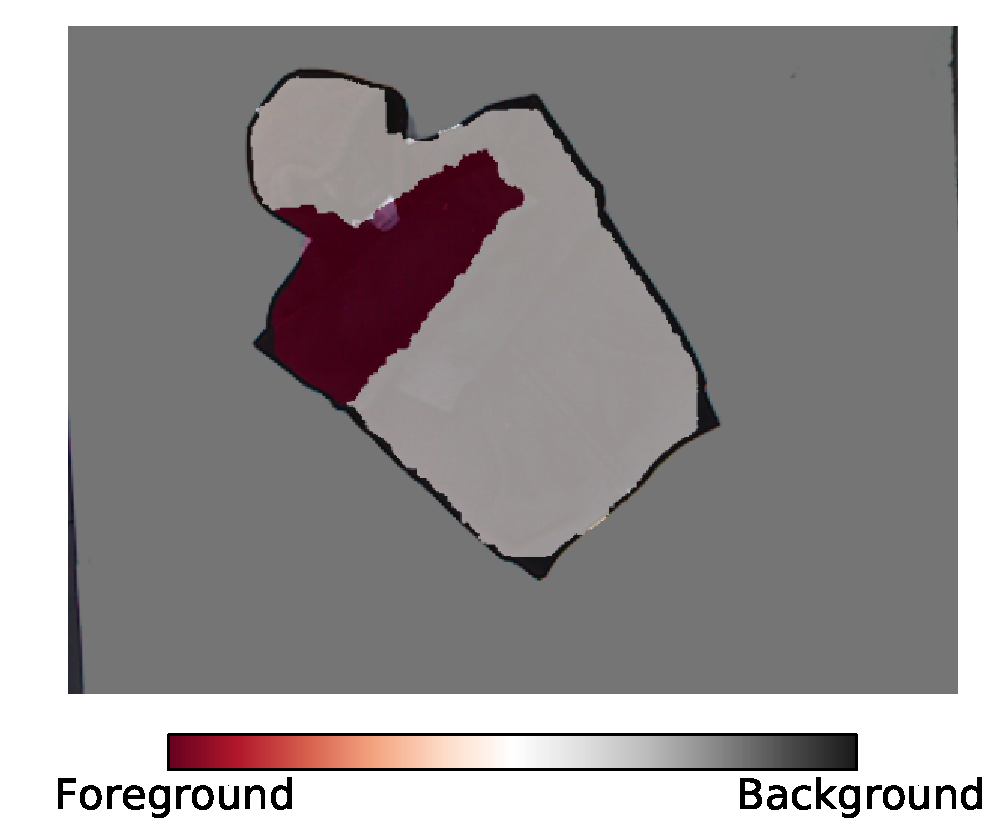
\includegraphics[width=\textwidth]
    	{figures/clustering/hoodie13-clustering.pdf}
	\end{subfigure}
	~
    \begin{subfigure}[r]{0.49\textwidth}
	    \centering
    	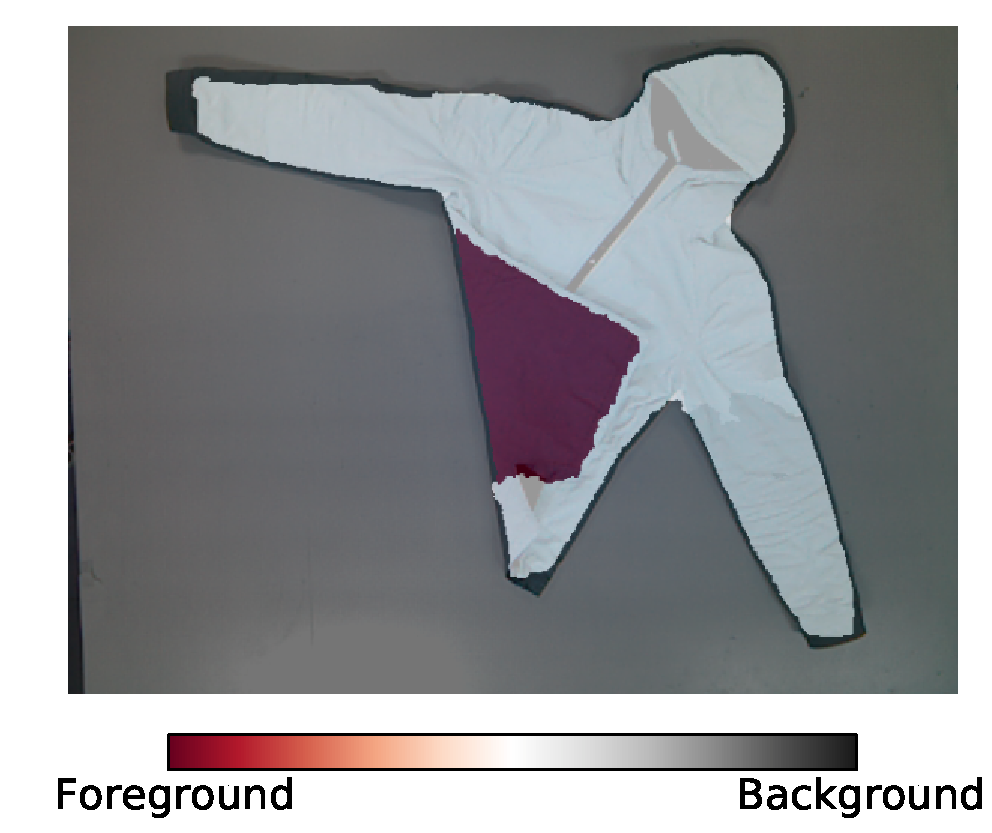
\includegraphics[width=\textwidth]
    	{figures/clustering/jacket7-clustering.pdf}
	\end{subfigure} 
	~
	\begin{subfigure}[l]{0.49\textwidth}
	    \centering
    	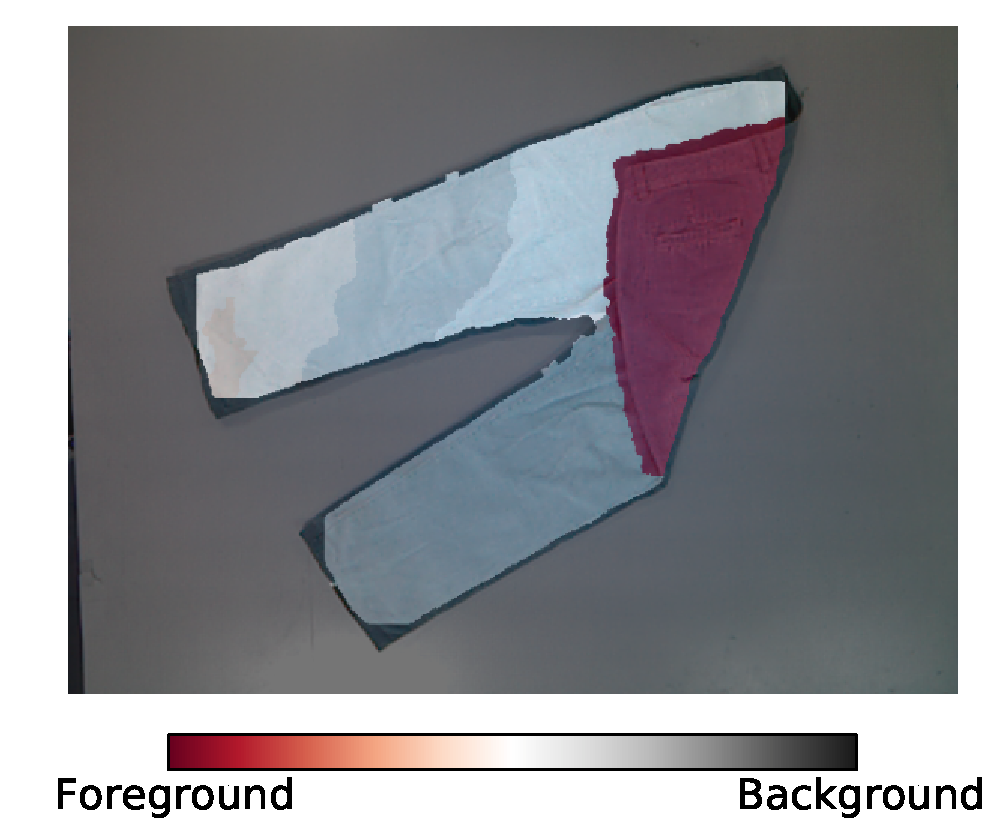
\includegraphics[width=\textwidth]
    	{figures/clustering/pants3-clustering.pdf}
	\end{subfigure}
	~
    \begin{subfigure}[r]{0.49\textwidth}
	    \centering
    	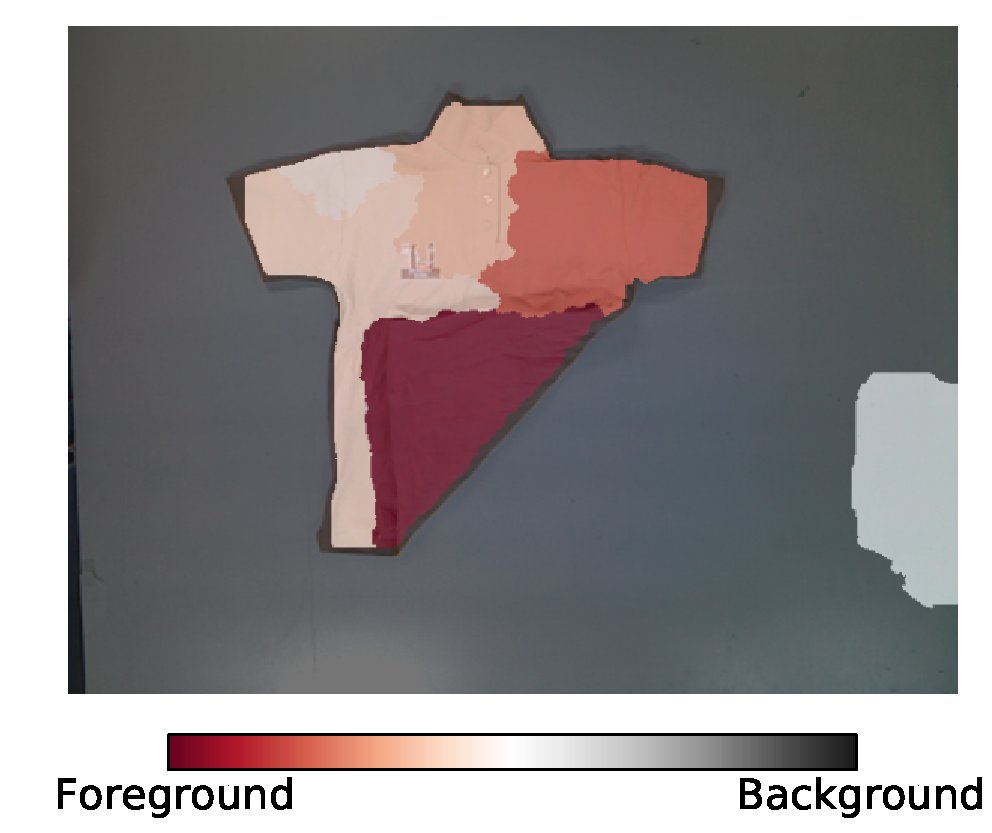
\includegraphics[width=\textwidth]
    	{figures/clustering/polo6-clustering.pdf}
	\end{subfigure}
	~
	\begin{subfigure}[l]{0.49\textwidth}
	    \centering
    	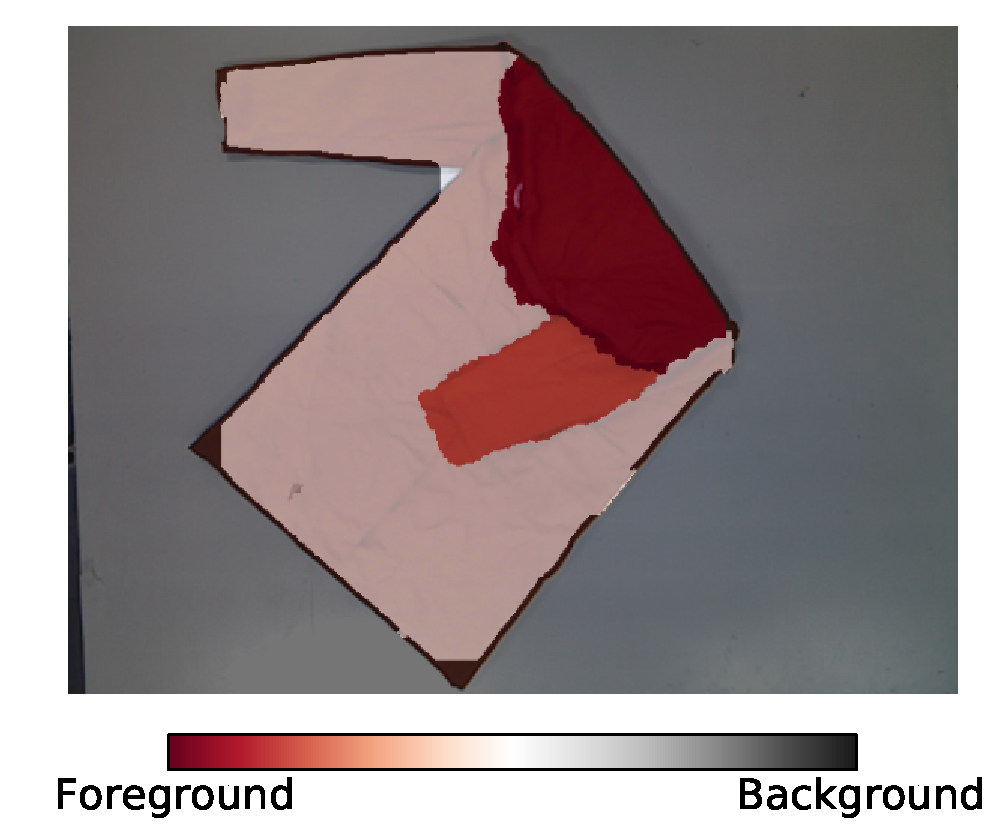
\includegraphics[width=\textwidth]
    	{figures/clustering/robe19-clustering.pdf}
	\end{subfigure}
	~
    \begin{subfigure}[r]{0.49\textwidth}
	    \centering
    	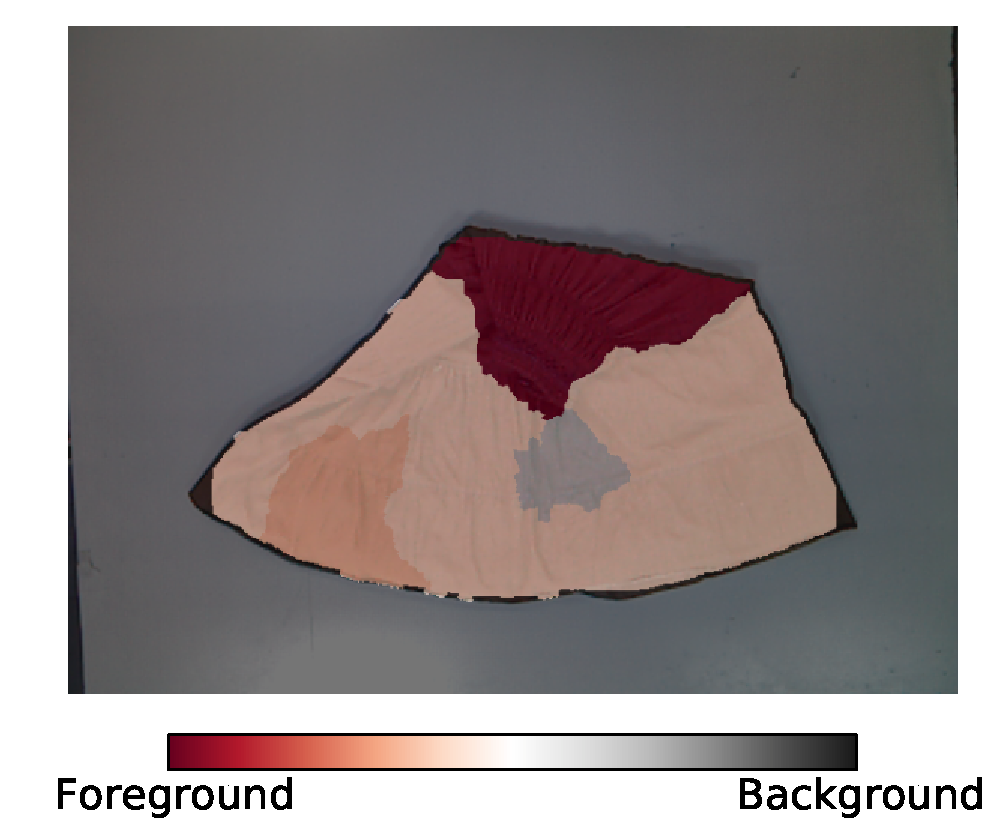
\includegraphics[width=\textwidth]
    	{figures/clustering/skirt17-clustering.pdf}
	\end{subfigure} 
    \caption[The normalized depth images for different clothes are shown on the left side.]
    {The normalized depth images for different clothes are shown on the left side. The grey level is related to the height of the point as detected by the RGB-D sensor. A darker grey level indicates the points are closer to the sensor. On the right side, the labeled image returned by watershed algorithm is presented, where each color represents a region of similar height.}
    \label{fig:watershed_labels}
\end{figure}